\documentclass[11pt,a4paper]{article}
\author{TalentSprint}
\date{}
\usepackage{verbatim}
\usepackage{fancyhdr}           % For header and footer
\usepackage{multicol}
\usepackage{colortbl}           % For coloured tables
\usepackage{setspace}           % For line height
\usepackage{seqsplit}           % Splits long words.
\usepackage{amsmath} 
\usepackage{graphicx}
\usepackage{array}
\usepackage{enumitem}
\usepackage{xcolor}
\usepackage[tikz]{bclogo}
\usepackage{textcomp}
\usepackage{listings}
\lstset{language=python,numbers=left,numberstyle=\tiny,numbersep=10pt,showstringspaces=false}

\headheight=14pt
\lhead{\nouppercase{}}
\rhead{\nouppercase{\leftmark}}

\graphicspath{{../Images/} {../ScreenShots/}}
\setcounter{tocdepth}{1}
\setlength\parindent{0pt}
\parskip=4pt
\newcommand{\Code}[1]{\textbf{\texttt{#1}}}

\begin{comment}
\def\AnswerBox{\fbox{\begin{minipage}{4in}\hfill\vspace{0.5in}\end{minipage}}}
\newcommand{\Code}[1]{\textbf{\texttt{#1}}}
\thispagestyle{empty}
\vspace{1.5pc}
\topskip0pt
\vspace*{\fill}
\centerline{\Huge Modern Programming}
\vspace{2pc}
\centerline{\Huge Practice}
\vspace{2pc}
\centerline{\Large using Python}
\vspace*{\fill}
\centerline{Prepared by TalentSprint WISE Team} 
\setcounter{page}{1}
\pagestyle{fancy}

\end{comment}
%========================================================================

% Lengths and widths
\addtolength{\textwidth}{5cm}
\addtolength{\hoffset}{-1cm}
\setlength{\headsep}{-12pt} % Reduce space between header and content
\setlength{\headheight}{85pt} % If less, LaTeX automatically increases it
\renewcommand{\footrulewidth}{2pt} % Remove footer line
\renewcommand{\headrulewidth}{1pt} % Remove header line
\renewcommand{\seqinsert}{\ifmmode\allowbreak\else\-\fi} % Hyphens in seqsplit
% This two commands together give roughly
% the right line height in the tables
\renewcommand{\arraystretch}{1.3}
\onehalfspacing



% Commands
\newcommand{\SetRowColor}[1]{\noalign{\gdef\RowColorName{#1}}\rowcolor{\RowColorName}} % Shortcut for row colour
\newcommand{\mymulticolumn}[3]{\multicolumn{#1}{>{\columncolor{white}}#2}{#3}} % For coloured multi-cols
\newcolumntype{x}[1]{>{\raggedright}p{#1}} % New column types for ragged-right paragraph columns
\newcommand{\tn}{\tabularnewline} % Required as custom column type in use

% Font and Colours
\definecolor{HeadBackground}{HTML}{333333}
\definecolor{FootBackground}{HTML}{666666}
\definecolor{TextColor}{HTML}{333333}
\definecolor{DarkBackground}{HTML}{6B8E23} %{FD1AA8}
\definecolor{LightBackground}{HTML}{E8FED8} %D3FDC8
\definecolor{tit}{HTML}{FF6600}
\renewcommand{\familydefault}{\sfdefault}
\color{TextColor}
 \headsep = 25pt
% Header and Footer
\pagestyle{fancy}
\usepackage[headheight=110pt]{geometry}
\fancyhf{}% Clear header/footer

\fancyhead[r]{
\includegraphics[width = 4cm, height = 2cm]{TS-Logo.png}\hspace{0cm}}

%=================================TITLE=====================================
\fancyhead[l]{\Large{\bf{\textcolor{tit}{\textrm{Introduction to Python}}}}}
%===========================================================================

\renewcommand{\headrulewidth}{0.4pt}% Default \headrulewidth is 0.4pt
\renewcommand{\footrulewidth}{0.4pt}% Default \footrulewidth is 0pt

\rfoot{Page \thepage}
\lfoot{COPYRIGHT \textcopyright TALENTSPRINT, 2015. ALL RIGHTS RESERVED.}




\begin{document}



%\chapter*{Introduction to Python}
\section*{History}

Python was developed in the late 1980's by Guido van Rossum. The first release was version 0.90 in February, 1991, at the National Research Institute for Mathematics and Computer Science in the Netherlands. The Institute is more popularly known by the Dutch name and initials Centrum Wiskunde and Informatica--CWI. \footnote{CWI is famous for its association with Adriaan van Wijngaarden and Edsger Dijkstra.}

It is derived from many languages like ABC, C, Unix shell and other scripting languages. But its primary influence in the early stages was ABC and the desire to design an easy to learn, first language for learning programming.

Since 2001, the Python Software Foundation (PSF) a non-profit organization, created specifically to own Python-related Intellectual Property, directs the development, evangelising and directions of the language.

Guido van Rossum continues to be the prime mover and is fondly referred to as BDFL--Benevolent Dictator For Life.

\section*{What is Python}
Python is a high-level, interpreted, interactive and object-oriented language. Its hallmark is an elegant syntax that enables writing very easy to read programs.

\subsection*{Notable features}
\begin{itemize}
    \item Uses an elegant syntax, making the programs you write easier to read.
    \item Makes it easy to get your program working -- ideal for prototype development and other ad-hoc programming tasks, without compromising maintainability.
    \item Comes with a large standard library that supports many common programming tasks such as connecting to web servers, searching text with regular expressions, reading and modifying files. Often referred to as \emph{batteries included} feature of Python.
    \item Runs on many different computers and operating systems: Windows, MacOS, many brands of Unix, OS/2, \ldots
    \item Has excellent Unicode support.
\end{itemize}   

\subsection*{Language characteristics}
    \begin{itemize}
        \item All basic data types are available: numbers (floating point, complex, and unlimited-length integers), strings.
        \item Higher level containers such as  lists, dictionaries and sets are part of the core language.
        \item Python supports object-oriented programming with classes and multiple inheritance.
        \item Modules and packages are the mechanisms to design, build, and distribute applications and libraries.
        \item Exception handling is available. 
        \item Data types are strongly and dynamically typed. Mixing incompatible types (e.g. attempting to add a string and a number) causes an exception to be raised, so errors are caught sooner.
        \item Provides advanced programming features such as generators and list comprehensions.
        \item Automatic memory management frees you from having to manually allocate and free memory in your code.
    \end{itemize}

    \section*{Application Areas}
    Python has now become a widely used professional language; it is used by organizations such as Google, NASA, Industrial Light and Magic, Cerenova, ABN Amro Bank \ldots

    The following is a partial list of tools, frameworks and applications developed in python.

    \begin{description}
    \item[Web Development] Python offers many choices for web development:
        \begin{itemize}
            \item Full-stack frameworks such as Django, Pyramid, and Zope.
            \item Micro-frameworks such as Flask and Bottle.
            \item Advanced content management systems such as Plone.
            \item Python's standard library supports many Internet protocols:
                \begin{itemize} 
                    \item HTML, XML, JSON.
                    \item E-mail processing.
                    \item FTP, IMAP, sockets \ldots
                \end{itemize}
            \item Requests, a powerful HTTP client library.
            \item BeautifulSoup, a `fault-tolerant' HTML parser.
            \item Feedparser for parsing RSS/Atom feeds.
            \item Paramiko implements the SSH2 protocol.
            \item Twisted Python, for asynchronous network programming.
        \end{itemize}
    \item[Scientific Computation] Python is widely used in scientific and engineering computing. In fact it has become the de-facto standard toolkit for such work. 
    \begin{itemize}
        \item SciPy is \textbf{the} collection packages for mathematics, science, and engineering.
        \item Pandas is a data analysis and modeling library.
        \item IPython is currently leading the effort at providing an interactive computation and exploration platform.
    \end{itemize}
\item[Education] Python is ideal for teaching programming, both at the introductory level and in more advanced courses. The most famous of the MIT's courses, 6.00x, switched to using Python a few years back.
\item[GUI Toolkits] Python has wide variety of graphical interface libraries.
    \begin{itemize} 
        \item The Tk GUI library is included with Python.
        \item wxWidgets is a powerful big multiplatform gui toolkit
        \item Kivy, for writing multitouch applications, on say Android
        \item Qt can be used via pyqt or pyside libraries
    \end{itemize}
    \end{description}

\section*{Versions and Implementations}
The canonical reference implementation of the python language is what is mostly used. This is written in C and is the one originally developed by Guido van Rossum. When required to distinguish this from other implementations the term \emph{CPython} is used to refer to it.

One of the earliest implementations is  called Jython--as you can guess it is implemented in Java and is quite prpular among companies that are predominantly Java based, but like to use Python in appropriate areas.

On the .NET platform there is IronPython. 

Pypy is an interesting attempt to implement Python in Python! It provides an optimising JIT compiler.

There are two major versions of Python currently in use. 2.7 and 3.3. Python 3 is backward incompatible effort to clean up some of the errors and inconsisitencies in the original implementation. 

We will use Python 3.3 in our course.

\section*{Tool Set}
There are many ways to create Python programs:
\begin{description}
    \item[1. Interactive Interpreter] You can start the interpreter just by giving the name \texttt{python3}\footnote{In most Linux distributions, Python 2.x is by default installed with the executable named \texttt{python}. So python 3.x executable is installed as \texttt{python3}. This expected to change over time. In some distributions, such as ArchLinux, python3 is the default and you have to run python2 by typing \texttt{python2}.}

Once Python has started, you will see the interpreter startup message indicating version and platform and be given the interpreter prompt ``$>>>$'' to enter commands.

\begin{figure}[ht]
\begin{center}
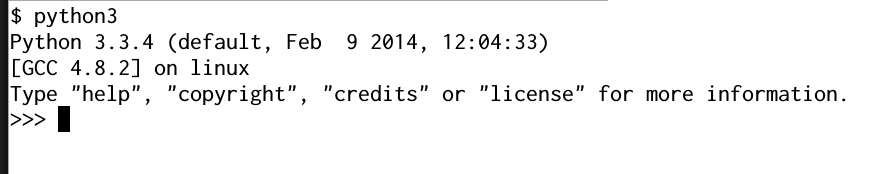
\includegraphics[scale=0.5]{01-Interpreter.png}
\caption{Interpreter - Linux}
\label{Interpreter}
\end{center}
\end{figure}

\item[2. Writing Script on file] Follow these steps to write and execute a script.
\begin{itemize}
    \item At the (\$) prompt create a file using vim (or any text editor),\\\texttt{\$ vim filename.py}.
    \item Write code in the file save it.
\item Execute - come back to terminal and type \texttt{\$ python filename.py} it generates the output in the console
\end{itemize}
As you can gather python programs have the extension \texttt{.py}

\item[3. Integrated Development Environment] We can also use graphical Interactive Development Environment - IDE to enter, and run python programs. The default ide in Linux is called \emph{IDLE}

IDLE is the basic editor and interpreter environment with standard distribution of python. It looks like,

\begin{figure}[ht]
\begin{center}
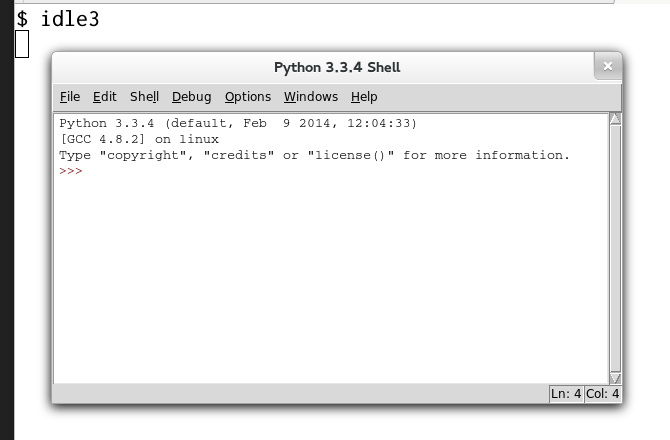
\includegraphics[scale=0.5]{02-IDLE.png}
\caption{IDLE}
\label{IDLE}
\end{center}
\end{figure}

\item[4. Using iPython] Our preferrred interactive environment is called iPython. It is invoked by typing \texttt{ipython3} at the \$ prompt. 
\begin{figure}[ht]
\begin{center}
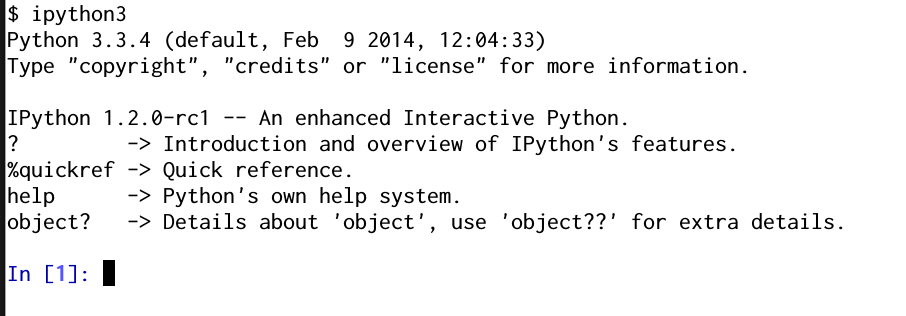
\includegraphics[scale=0.5]{03-iPython.png}
\caption{iPython}
\label{ipython}
\end{center}
\end{figure}

The reason we prefer iPython is that it provides much more help interactively.

\section*{Sample Program}
Now let us write our first Python program. The program will display a message: \emph{Welcome to the World of  Python}

Let us open the terminal and run the python interpreter: that is type python3 at the \$prompt. At the $>>>$ prompt type the line (and hit ENTER).

\texttt{$>>>$ print("Welcome to the World Of Python")}

It produces the following result:

\texttt{Welcome to the World of Python}

Now let us write the same program in a script.

\begin{enumerate}
    \item Open the file using \textbf{\texttt{\$ vim Program-01-1.py}} and type the following line and save the file.

\texttt{print("Welcome to the World Of Python")}

\item Now type the below command in terminal and press Enter Key to Execute.
\end{enumerate}
\texttt{\$ python Program-01-1.py }

%\texttt{Welcome to the World of Python}
\subsection*{Output}

\begin{figure}[ht]
\begin{center}
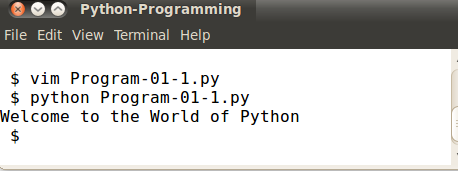
\includegraphics[scale=0.6]{Output-Program-01-1.png}
\end{center}
\end{figure}

\end{description}

\begin{bclogo}[couleur=blue!5, arrondi=0.3, logo=\bctrombone]{Note}
Recall that python is an interpreted language. So the execution takes place without any compiling, linking or producing an executable.
\end{bclogo}

\section*{Building blocks of Python Program}
In order to understand the functioning of a program, we need to understand the role of the following elements. It should be noted that this perspective is in no way intended as describing the structure of a program. 
\begin{description}
\item [Functions] Functions are the main building blocks of any programming language. Unlike C, python does not have a \texttt{main()} function to begin. We will discuss functions in detail later.
\item [Variables] Variables are very flexible. You do not have to declare them first, like in other languages like C . You can assign any value to them, even if they already have a value of a different type.
\item [Expressions] An expression is a combination of variables, operators and values which represents a single result value.
\item [Statements] Statements can be expressions, assignments, function calls, or control flow statements which make up python program.
\item [Block] A block is a lexical grouping of statements and can be thought of as \emph{one} logical statement. A block in python is delimited by indentation.
\item [Comments] Comments start with  the hash character `\#', and extend to end of the line. A comment may appear at the start of the line or following white space  or code, but  not within a string literal. A hash character within a string literal is just a hash character. Since comments are to clarify code and are not interpreted by Python, they can be omitted.
\end{description}


\section*{Naming Rules in Python}
There are a few set of rules for choosing variable names:
\begin{itemize}
\item Must begin with a alphabet(a - z, A - Z) or underscore(\_).
\item Other characters can be alphabets, digits or underscore(\_).
\item Python is case sensitive; uppercase and lower case alphabets are treated as distinct.
\end{itemize}

You should ensure that you use meaningful names for your identifiers. Please note meaningful \emph{does not} necessarily mean long. The goal is to make the program easier to read and be self-documenting. 

\section*{Keywords}
Keywords are reserved identifiers that have strict meaning which cannot be used as identifiers in the program. Note that some of the keywords are capitalized.
\texttt{
\begin{table}[h]
\centering
\begin{tabular}{l l l l}\\
and  & elif & import & return\\
as & else & in & try\\
assert & except & is & while\\
break & finally & lambda & with\\
class & for & not & yield\\
continue & from & or & True\\
def & global & pass & False\\
del &  if  & raise & None\\ 
\end{tabular}
\caption{List of Python keywords}
\end{table}
}

\section*{Additional notes}
 
\[
  \left[
      \begin{tabular}{@{\quad}m{.3\textwidth}@{\qquad}m{.6\textwidth}@{\quad}}
        \includegraphics[width=\linewidth]{Python-Logo.jpg} &
          \raggedright%
          \textbf{Origin of the name} \par
          Though the logo is a stylized representation of the reptile, the language is \emph{NOT} named after a snake, but a famous British comedian Monty Python -- Guido is a great fan!
      \end{tabular}
    \right]
\]


\end{document}
